% !TEX program = lualatex
\documentclass[aspectratio=43,professionalfonts,handout]{beamer}
\usepackage{beamer_template}

\newcommand{\LectureNum}{11}
\newcommand{\LectureTitle}{分数関数（２）}
\newcommand{\TextPages}{p.\,93}
\newcommand{\NextTopic}{無理関数}
\newcommand{\NextPages}{p.\,94-95}
\newcommand{\CourseName}{基礎数学B}
\renewcommand{\TermName}{前期}

\begin{document}

% -----------------------------------------------
% スライド1: 表紙＋目標＋用語・定義
% -----------------------------------------------
\begin{frame}{\CourseName\quad 第\LectureNum 回「\LectureTitle 」}
  {\small \TermName\quad \TeacherName\quad ／\quad 教科書 \TextPages\quad
  \textbf{目標}：y=(cx+d)/(x+b) 型の分数関数のグラフを描ける}

  \begin{block}{用語・定義}
  \begin{description}[labelwidth=5.5em]
    \item[\kw{変形の方針（分子÷分母）}] ~
    \item[\kw{漸近線の読み取り方}] ~
  \end{description}
  \end{block}
\end{frame}

% -----------------------------------------------
% スライド2: 公式・性質
% -----------------------------------------------
\begin{frame}{公式・性質}
  \begin{block}{}
  \begin{itemize}
    \item y=(cx+d)/(x+b) → y=c+(d-bc)/(x+b) の変形手順
    \item 例：(3x+7)/(x+2) = 3+1/(x+2)
  \end{itemize}
  \end{block}
\end{frame}

% -----------------------------------------------
% スライド3: 図・グラフ（TikZコードを手動追加）
% -----------------------------------------------
\begin{frame}{図・グラフ}
  \centering
  % TODO: y=(3x+7)/(x+2) のグラフと漸近線 x=-2、y=3
  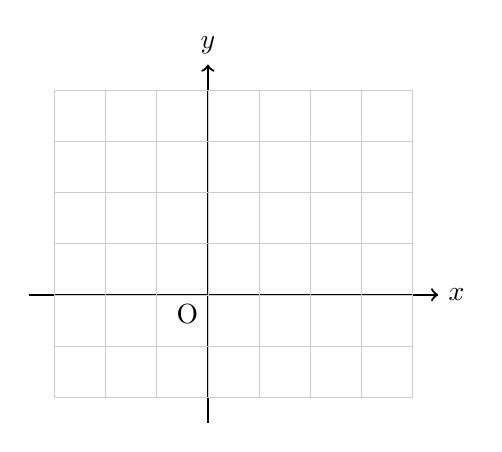
\begin{tikzpicture}[scale=0.65]
    \draw[->,thick] (-3.5,0) -- (4.5,0) node[right]{$x$};
    \draw[->,thick] (0,-2.5) -- (0,4.5) node[above]{$y$};
    \node[below left] at (0,0) {O};
    \draw[gray!40, very thin] (-3,-2) grid (4,4);
    % ここにグラフを描画
  \end{tikzpicture}
\end{frame}

% -----------------------------------------------
% スライド4: 例1→問1
% -----------------------------------------------
\begin{frame}{例1→問1}
  \begin{exampleblock}{例) p.93（変形とグラフ）}
    （板書で解説）
  \end{exampleblock}

  \vfill

  \begin{block}{問4) p.93（2問）\quad 自分で解いてみよう}
    （ノートに解くこと）
  \end{block}
\end{frame}

% -----------------------------------------------
% スライド5: 例2→問2
% -----------------------------------------------
\begin{frame}{例2→問2}
  \begin{exampleblock}{練習2-A 問4) p.99（係数を求める）}
    （板書で解説）
  \end{exampleblock}

  \vfill

  \begin{block}{練習2-B 問4) p.100\quad 自分で解いてみよう}
    （ノートに解くこと）
  \end{block}
\end{frame}

% -----------------------------------------------
% まとめ
% -----------------------------------------------
\begin{frame}{まとめ}
  \begin{itemize}
    \item y=(cx+d)/(x+b) は分子÷分母で y=q+r/(x+b) に変形する
    \item 変形後の形から漸近線を読み取り、双曲線をかく
  \end{itemize}

  \vfill
  {\small 基本問題：174}
\end{frame}

\end{document}
